% DPF 09 talk on strangeness in nucleon

\documentclass[10pt]{beamer}
\usepackage{amsmath}
\usepackage{mathtools}
%\documentclass[12pt]{beamerthemeSam.sty}
\usepackage{epsf}
%\usepackage{pstricks}
%\usepackage[orientation=portrait,size=A4]{beamerposter}
\geometry{paperwidth=160mm,paperheight=120mm}
%DT favorite definitions
\def\LL{\left\langle}	% left angle bracket
\def\RR{\right\rangle}	% right angle bracket
\def\LP{\left(}		% left parenthesis
\def\RP{\right)}	% right parenthesis
\def\LB{\left\{}	% left curly bracket
\def\RB{\right\}}	% right curly bracket
\def\PAR#1#2{ {{\partial #1}\over{\partial #2}} }
\def\PARTWO#1#2{ {{\partial^2 #1}\over{\partial #2}^2} }
\def\PARTWOMIX#1#2#3{ {{\partial^2 #1}\over{\partial #2 \partial #3}} }

\def\rightpartial{{\overrightarrow\partial}}
\def\leftpartial{{\overleftarrow\partial}}
\def\diffpartial{\buildrel\leftrightarrow\over\partial}

\def\BI{\begin{itemize}}
\def\EI{\end{itemize}}
\def\BE{\begin{displaymath}}
\def\EE{\end{displaymath}}
\def\BEA{\begin{eqnarray*}}
\def\EEA{\end{eqnarray*}}
\def\BNEA{\begin{eqnarray}}
\def\ENEA{\end{eqnarray}}
\def\EL{\nonumber\\}


\newcommand{\map}[1]{\frame{\frametitle{\textbf{Course map}}
\centerline{\includegraphics[height=0.86\paperheight]{../../map/#1.png}}}}
\newcommand{\wmap}[1]{\frame{\frametitle{\textbf{Course map}}
\centerline{\includegraphics[width=0.96\paperwidth]{../../map/#1.png}}}}

\newcommand{\etal}{{\it et al.}}
\newcommand{\gbeta}{6/g^2}
\newcommand{\la}[1]{\label{#1}}
\newcommand{\ie}{{\em i.e.\ }}
\newcommand{\eg}{{\em e.\,g.\ }}
\newcommand{\cf}{cf.\ }
\newcommand{\etc}{etc.\ }
\newcommand{\atantwo}{{\rm atan2}}
\newcommand{\Tr}{{\rm Tr}}
\newcommand{\dt}{\Delta t}
\newcommand{\op}{{\cal O}}
\newcommand{\msbar}{{\overline{\rm MS}}}
\def\chpt{\raise0.4ex\hbox{$\chi$}PT}
\def\schpt{S\raise0.4ex\hbox{$\chi$}PT}
\def\MeV{{\rm Me\!V}}
\def\GeV{{\rm Ge\!V}}

%AB: my color definitions
%\definecolor{mygarnet}{rgb}{0.445,0.184,0.215}
%\definecolor{mygold}{rgb}{0.848,0.848,0.098}
%\definecolor{myg2g}{rgb}{0.647,0.316,0.157}
\definecolor{abtitlecolor}{rgb}{0.0,0.255,0.494}
\definecolor{absecondarycolor}{rgb}{0.0,0.416,0.804}
\definecolor{abprimarycolor}{rgb}{1.0,0.686,0.0}
\definecolor{Red}           {cmyk}{0,1,1,0}
\definecolor{Grey}           {cmyk}{.7,.7,.7,0}
\definecolor{Blue}          {cmyk}{1,1,0,0}
\definecolor{Green}         {cmyk}{1,0,1,0}
\definecolor{Brown}         {cmyk}{0,0.81,1,0.60}
\definecolor{Black}         {cmyk}{0,0,0,1}

\usetheme{Madrid}


%AB: redefinition of beamer colors
%\setbeamercolor{palette tertiary}{fg=white,bg=mygarnet}
%\setbeamercolor{palette secondary}{fg=white,bg=myg2g}
%\setbeamercolor{palette primary}{fg=black,bg=mygold}
\setbeamercolor{title}{fg=abtitlecolor}
\setbeamercolor{frametitle}{fg=abtitlecolor}
\setbeamercolor{palette tertiary}{fg=white,bg=abtitlecolor}
\setbeamercolor{palette secondary}{fg=white,bg=absecondarycolor}
\setbeamercolor{palette primary}{fg=black,bg=abprimarycolor}
\setbeamercolor{structure}{fg=abtitlecolor}

\setbeamerfont{section in toc}{series=\bfseries}

%AB: remove navigation icons
\beamertemplatenavigationsymbolsempty
\title[Universal gravitation]{
  \textbf {Universal gravitation}\\
%\centerline{}
%\centering
%\vspace{-0.0in}
%\includegraphics[width=0.3\textwidth]{propvalues_0093.pdf}
%\vspace{-0.3in}\\
%\label{intrograph}
}

\author[W. Freeman] {Physics 211\\Syracuse University, Physics 211 Spring 2015\\Walter Freeman}

\date{\today}

\begin{document}

\frame{\titlepage}

\frame{\frametitle{\textbf{Announcements}}
\BI
\large
\item{I crashed my car on Thursday -- sorry for late answers to emails}
  \BI
\item{I'm a bit behind on regrades -- there's a huge stack, but I haven't forgotten them}
  \EI
\item{Homework 5 (short) due Friday}
\item{Practice exam posted}
  \BI
\item{Work on practice exam during recitations (and elsewhere)}
\item{Full solutions will be posted Friday}
  \EI
\item{{\bf Exam date moved} per your feedback to March 3}
\item{Exam prep schedule}
  \BI
\item{Wednesday: clinic hours by appointment/request (I'll be around most of the day)}
\item{Thursday: Review emphasizing basic things, 1:30-5PM, location TBA}
\item{Friday: Review 10AM-4PM, location TBA}
\item{\bf This is a huge amount of extra help available -- use it!}
  \EI
\EI

}

\frame{\frametitle{\textbf{Ask a Physicist: Poking a hole in the Earth}}
\Large
  
  ``If you drill a hole through the earth and jump into it, what would happen?''

\pause

\bigskip
\bigskip
\bigskip
\bigskip

Give me 30 minutes and I'll tell you, as we're doing gravity in general today!
}


\frame{\frametitle{\textbf{Gravity, in general}}
  \Large
  \BI
\item{On Earth all objects experience a gravitational force proportional to their mass:}
\item{$F_{\rm{grav}} = mg$, directed down toward the Earth}
  \BI
  \large
\item{How does this work when you're not on Earth?}
\item{What determines how big $g$ is?}
  \EI
  \EI
}

\frame{\frametitle{\textbf{A brief history of gravity and the heavens}}
\large
  The history here is an interesting insight into the way scientific thought has evolved:
``How can we explain the sky?''
\BI
\item{Stars in the sky all seem to move together, but with some ``wanderers'': planets}
  \BI
\item{They appear to move in one direction, but sometimes stop and turn around}

\bigskip

\centerline{  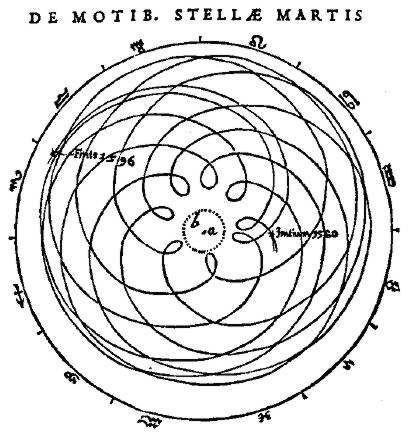
\includegraphics[width=0.3\textwidth]{Kepler_Mars_retrograde.jpg}}

  \bigskip
\item{How can we explain this?}
  \EI
  \EI
}
\frame{\frametitle{\textbf{A brief history of gravity and the heavens}}
\BI
\item{Ptolemy: Things go in circles rotating on circles, because circles are perfect, with the Earth at the center}
  \BI
\item{``Epicycles'' required to make the retrograde motion}
\EI
\item{Copernicus: Things go in circles rotating on circles, but with the Earth at the center}
  \BI
\item{Relative motion between Earth and planets responsible for retrograde motion}
  \EI
\item{Brahe: Fantastic measurements of motions of the planets (even more epicycles); geoheliocentrism}
\item{Kepler: Ellipses! No epicycles needed. Laws of planetary motion.}
\item{Galileo: Kinematics; moons of Jupiter; phases of Venus}
\item{Newton: Universal gravitation; dynamics}
  \EI
}

\frame{\frametitle{\textbf{Newtonian gravity}}
  \large
\BI
\item{All objects -- stars, planets, apples, people -- exert forces on each other}
\item{That force is given by}

  \bigskip
  
 \centerline{$F_g = \frac{GMm}{r^2}$}

\bigskip
\item{Both objects feel the same force, directed toward each other}
\item{Note:}

  \bigskip

    \centerline{$a_g = F_g/m = \frac{GM}{r^2}$}

    \bigskip

  \item{What is $G$?}
  \BI
\item{Fundamental constant of nature that tells us how strong gravity is}

  \bigskip

  \centerline{  \Large$G=6.673\times10^{-11} \frac{\rm N\cdot\rm m^2}{\rm{kg}^2}$}

\bigskip

\item{This is really, really tiny}
  \EI
  \EI
}

\frame{\frametitle{\textbf{Measuring $G$}}
  \centerline{  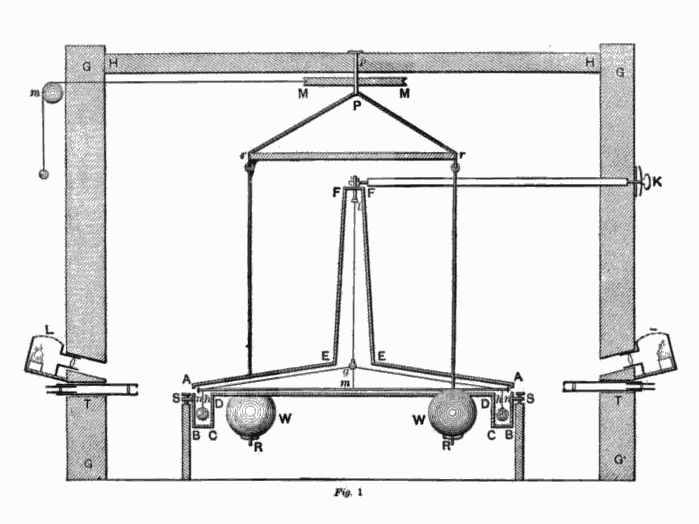
\includegraphics[width=0.8\textwidth]{Cavendish_Experiment.png}}

  \pause

  \centerline{\Large What is the force between a 1kg mass and a 5kg mass that are 5cm apart?}
}

\frame{\frametitle{\textbf{Measuring the mass of the Earth}}

  \Large \centerline{  What is the mass of the Earth?}

  \pause

\bigskip

  $F_g = \frac{GMm}{r^2} = mg$


  \bigskip

  \pause

  $M = \frac{gR^2}{G} = 5.97 \times 10^{24}$ kg...
}

\frame{\frametitle{\textbf{Gravity and circular motion}}
  \Large
  \begin{itemize}
    \item{Many orbits are nearly circular}
    \item{Everything you learned on Tuesday about uniform circular motion still applies}
    \item{Weighing the Earth by looking at the Moon:}
      \BI
      \Large
    \item{$F_g = \frac{GM_e M_m}{r^2} = M_m \omega^2 r$}
      \EI
    \item{These problems are nothing new and nothing hard; it's just a new force}
      \EI
}

\frame{\frametitle{\textbf{Kepler's law: relation of orbital period to radius}}
  \Large
  \begin{center}
$F_g = \frac{GMm}{r^2}$

\bigskip\pause

$m\omega^2 r = \frac{GMm}{r^2}$

\bigskip\pause

$r^3 \omega^2 = GM$

\bigskip\pause

$T=\frac{2\pi}{\omega} \rightarrow \omega = \frac{2\pi}{T}$

\bigskip\pause

$\frac{4 \pi^2 r^3}{T^2} = GM$

\bigskip\pause

$\frac{r^3}{T^2} = \frac{GM}{4\pi^2}$
\end{center}
}

\frame{\frametitle{\textbf{Ask a Physicist: Digging a very deep hole...}}
  \large
    \BI
  \item{$g = \frac{GM}{r^2}$}
  \item{As you fell, you would get closer to the center of the Earth: $r$ decreases}
  \item{... but less of the Earth's mass would be under you: $M$ decreases too}
  \item{Remember the volume of a sphere: $V = \frac{4}{3} \pi r^3$}
  \item{$M \propto r^3$, so $g(r) \propto r$; as you fell your acceleration would decrease}
  \item{How fast are you going at the very center of the earth?}
    \EI
  }
\end{document}



